% !TEX program = pdflatex
% 固体物理第十三次作业
\documentclass[UTF8,10pt,a4paper]{article}
\usepackage{ctex}
% \catcode`\。=\active
% \newcommand{。}{.}
\newcommand{\CourseName}{固体物理}
\newcommand{\CourseCode}{PHYS1502}
\newcommand{\Semester}{2019-2020学年第二学期}
\newcommand{\ProjectName}{第十三次作业}
\newcommand{\DueTimeType}{截止时间}
\newcommand{\DueTime}{2020. 6. 5(周五)17:00}
\newcommand{\StudentName}{陈稼霖}
\newcommand{\StudentID}{45875852}
\usepackage[vmargin=1in,hmargin=.5in]{geometry}
\usepackage{fancyhdr}
\usepackage{lastpage}
\usepackage{calc}
\pagestyle{fancy}
\fancyhf{}
\fancyhead[L]{\CourseName}
\fancyhead[C]{\ProjectName}
\fancyhead[R]{\StudentName}
\fancyfoot[R]{\thepage\ / \pageref{LastPage}}
\setlength\headheight{12pt}
\fancypagestyle{FirstPageStyle}{
    \fancyhf{}
    \fancyhead[L]{\CourseName\\
        \CourseCode\\
        \Semester}
    \fancyhead[C]{{\Huge\bfseries\ProjectName}\\
        \DueTimeType\ : \DueTime}
    \fancyhead[R]{姓名 : \makebox[\widthof{\StudentID}][s]{\StudentName}\\
        学号 : \StudentID\\
        成绩 : \underline{\makebox[\widthof{\StudentID}]{}}}
    \fancyfoot[R]{\thepage\ / \pageref{LastPage}}
    \setlength\headheight{36pt}
}
\usepackage{amsmath,amssymb,amsthm,bm}
\allowdisplaybreaks[4]
\newtheoremstyle{Problem}
{}
{}
{}
{}
{\bfseries}
{.}
{ }
{第\thmnumber{ #2}\thmname{ #1}\thmnote{ (#3)} 得分: \underline{\qquad\qquad}}
\theoremstyle{Problem}
\newtheorem{prob}{题}
\newtheoremstyle{Solution}
{}
{}
{}
{}
{\bfseries}
{:}
{ }
{\thmname{#1}}
\makeatletter
\def\@endtheorem{\qed\endtrivlist\@endpefalse}
\makeatother
\theoremstyle{Solution}
\newtheorem*{sol}{解}
\providecommand{\abs}[1]{\left\lvert#1\right\rvert}
\usepackage{graphicx}
\begin{document}
\thispagestyle{FirstPageStyle}
\begin{prob}[(18.1) Semiconductor Quantum Well]
    \begin{enumerate}
        \item[(a)] A quantum well is from a layer of GaAs of thickness $L$ nm, surrounded by layers of Ga$_{1-x}$Al$_x$As (See Fig. 18.2). You may assume that the band gap of the Ga$_{1-x}$Al$_x$As is substantially larger than that of GaAs. The electron effective mass in GaAs is $0.068m_e$ whereas the hole of effective mass is $0.45m_e$ with the $m_e$ the mass of the electron.
        \begin{itemize}
            \item[$\triangleright$] Sketch the shape of the potential for the electrons and holes.
            \item[$\triangleright$] What approximate value of $L$ is required if the band gap of the quantum well is to be $0.1$ eV larger than that of GaAs bulk material?
        \end{itemize}
        \item[(b)$^*$] What might this structure be useful for?
    \end{enumerate}
\end{prob}
\begin{sol}
    \begin{enumerate}
        \item[(a)]
        \begin{itemize}
            \item[$\triangleright$] 被禁锢在量子阱中的载流子可被近似视为被约束在无限深方势阱中的载流子,其能级是分立的,其中电子的能级为
            \begin{align}
                E_{e,l}=E_c+\frac{\hbar^2}{2m_e^*}\left(\frac{l\pi}{L}\right)^2,
            \end{align}
            其中$E_c$是块状GaAs导带最低点的能量,$l=1,2,3,\cdots$是能级序号.\\
            载流子的能级为
            \begin{align}
                E_{h,m}=\abs{E_v}+\frac{\hbar^2}{2m_h^*}\left(\frac{m\pi}{L}\right)^2
            \end{align}
            其中$E_v$是块状GaAs价带最高点的能量,$m=1,2,3,\cdots$是能级序号. 注意,对于载流子,处于价带上的能量应该都是正值,当然,下面我们画的能带结构中,纵坐标的正负都是相对于电子而言的. 该量子阱的能带结构如图\ref{1-bandstructure}所示.
            \begin{figure}[h]
                \centering
                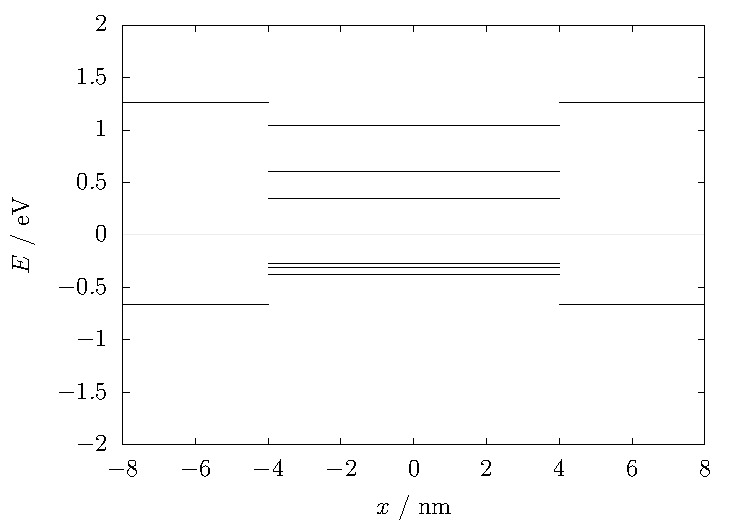
\includegraphics[width=.5\textwidth]{1-bandstructure.pdf}
                \caption{$L=8$nm时量子阱的能带结构,中间是GaAs的分立能级,两边为Ga$_{1-x}$Al$_x$As的能带(连续的). 注意横坐标是距离而非动量. 纵坐标的大小的绝对大小可能有不准确的offset(也就是说$E=0$不是准确的费米面),但其相对大小是准确的.}
                \label{1-bandstructure}
            \end{figure}
            \item[$\triangleright$] 欲使该量子阱的带隙(即一对导带上的电子和价带上的空穴合并所释放的能量)比块状GaAs的带隙大$0.1$eV,则
            \begin{align}
                (E_{e,1}+E_{h,1})-(E_c-E_v)=\frac{\hbar^2}{2}\left(\frac{\pi}{L}\right)^2\left(\frac{1}{m_e^*}+\frac{1}{m_h^*}\right)=0.1\text{eV},
            \end{align}
            解得量子阱中GaAs的厚度应为
            \begin{align}
                L=7.99\text{nm}
            \end{align}
        \end{itemize}
        \item[(b)] 可以通过调节Ga$_{1-x}$Al$_x$As中$Al$的含量$x$来调节量子阱的深度,同时可以通过调节GaAs层的厚度来调节其带隙,这样可以制成任意输出频率的激光,或者显示屏的像素点.
    \end{enumerate}
\end{sol}

\begin{prob}[(18.3) $p-n$ Junction$^*$]
    Explain the origin of the depletion layer in an abrupt $p-n$ junction and discuss how the junction causes rectification to occur. Stating your assumptions, show tha the total width $w$ of the depletion layer of a $p-n$ junction is
    \[
        w=w_n+w_p
    \]
    where
    \[
        w_n=\left(\frac{2\epsilon_r\epsilon_0N_A\phi_0}{eN_D(N_A+N_D)}\right)^{1/2}
    \]
    and a similar expression for $w_p$. Here $\epsilon_r$ is the relative permittivity and $N_A$ and $N_D$ are the acceptor and donor densities per unit volume, while $\phi_0$ is the difference in potential across the $p-n$ junction with no applied voltage. You will have to use Poison's equation to calculate the form of $\phi$ give the presence of the ion charges in the depletion region.
    \begin{itemize}
        \item[$\triangleright$] Calculate the total depletion charge and infer how this changes when an addition voltage $V$ is applied.
        \item[$\triangleright$] What is the differential capacitance of the dipole and why might it be useful to use a diode as a capacitor in an electronic circuit?
    \end{itemize}
\end{prob}
\begin{sol}
    \textbf{耗尽区的来源}:当n型半导体和p型半导体相接触,由于n型半导体在导带上有较多的电子,而p型半导体在价带上有较多的空穴,n型半导体导带上的电子会扩散到p型半导体的价带上与空穴结合从而降低系统的能量;同时由于电子的转移,n型半导体在接触面附近留下正离子,p型半导体则在接触面附近则产生负离子,从而在接触面附近形成由n型半导体指向p型半导体的电场,这又驱动电子从p型半导体的价带向n型半导体的导带漂移,当载流子由n型半导体向p型半导体的转移达到一定程度,扩散作用和漂移作用达到平衡. 此时,在接触面附近的一定范围内,不存在任何载流子,这就是所谓的耗尽区.\\
    \textbf{整流的原理}:p-n结中的净电流是漂移电流和扩散电流之差. 内建电场引起由p端流向n端的漂移电流
    \begin{align}
        I_{\text{drift}}\propto e^{-(E_c-\mu)/k_BT}\approx e^{-E_g/k_BT}.
    \end{align}
    电子浓度差异引起由n端流向p端的扩散电流
    \begin{align}
        I_{\text{diff}}\approx\frac{1}{e^{(E-E_c)/k_BT}}\approx\frac{1}{e^{E_g/k_BT}+1}\approx e^{-E_g/k_BT}.
    \end{align}
    当施加正偏压,扩散电流变为
    \begin{align}
        I_{\text{drift}}\approx e^{-(E_g-eV)/k_BT},
    \end{align}
    其中$V>0$. 通过p-n结的净电流为
    \begin{align}
        I=I_{\text{diff}}-I_{\text{drift}}\approx e^{-E_g/k_BT}(e^{eV/k_BT}+1).
    \end{align}
    可见当施加正弦偏压时,净电流随着电压的增大迅速增大. 当施负偏压,$V<0$,净电流将会变得很小. 这就是p-n结整流的原理.
    \begin{itemize}
        \item[$\triangleright$] 在耗尽区,没有载流子,只有固定不动的、均匀分布的正负离子,因此当地的电荷密度为
        \begin{align}
            \rho(x)=\left\{\begin{array}{ll}
                eN_D,&x<0,\\
                -eN_A,&x>0,
            \end{array}\right.
        \end{align}
        其中$x=0$对应着p型半导体和n型半导体的交界处,$x<0$区域是n型半导体(耗尽层留下阳离子),$x>0$区域是p型半导体(耗尽层留下阴离子),$N_D$是n型半导体中施主原子的线密度,$D_A$是p型半导体中受主原子的线密度(注意,是线密度,即每单位长度上的原子数目,否则量纲不对!!).
        求解泊松方程
        \begin{align}
            \frac{\partial^2\phi}{\partial x^2}=-\frac{\rho}{\epsilon_0\epsilon_r},
        \end{align}
        (为了得到题目中的结论,这里假定了n型半导体和p型半导体的介电常数相等,实际上两者一般不相等)\\
        就会得到如下形式的电势分布
        \begin{align}
            \phi(x)=\left\{\begin{array}{ll}
                -\frac{eN_D}{2\epsilon_0\epsilon_r}+C_Dx,&x<0,\\
                \frac{eN_A}{2\epsilon_0\epsilon_r}+C_Ax,&x>0
            \end{array}\right.
        \end{align}
        其中$C_D$和$C_A$是常数.
        若设n型半导体和p型半导体的耗尽层厚度分别为$w_n$和$w_p$,耗尽层的两端内建电场均为零,则上面的电势分布具有边界条件
        \begin{align}
            \frac{\partial\psi}{\partial x}(-w_n)=\frac{\partial\psi}{\partial x}(w_p)=0,
        \end{align}
        从而
        \begin{align}
            \phi(x)=\left\{\begin{array}{ll}
                -\frac{eN_D}{2\epsilon_0\epsilon_r}(x^2+w_nx),&x<0,\\
                \frac{eN_A}{2\epsilon_0\epsilon_r}(x^2-w_px),&x>0.
            \end{array}\right.
        \end{align}
        耗尽区两端的电势差为
        \begin{align}
            \phi_0=\phi(-w_n)-\phi(w_p)=\frac{e}{2\epsilon_0\epsilon_r}\left(N_Dw_n^2+N_Aw_p^2\right).
        \end{align}
        同时,考虑到p-n结在接触之前是电中性的,由于电荷的守恒,载流子转移平衡后,耗尽区中仍然应该是电中性的:
        \begin{align}
            w_pN_A=w_nN_D.
        \end{align}
        联立上面两式,得到n型半导体和p型半导体中耗尽区宽度分别为
        \begin{align}
            \nonumber w_n=&\left(\frac{2\epsilon_0\epsilon_rN_A\phi_0}{eN_D(N_A+N_D)}\right)^{1/2},\\
            \nonumber w_p=&\left(\frac{2\epsilon_0\epsilon_rN_D\phi_0}{eN_E(N_A+N_D)}\right)^{1/2}.
        \end{align}
        当在p-n结上施加一外加电压$V$,耗尽区两端的电势差由$\phi_0$变为$\phi_0+V$,用相同的方法n型半导体和p型半导体中耗尽区宽度分别为
        \begin{align}
            \nonumber w_n=&\left(\frac{2\epsilon_0\epsilon_rN_A(\phi_0+V)}{eN_D(N_A+N_D)}\right)^{1/2},\\
            \nonumber w_p=&\left(\frac{2\epsilon_0\epsilon_rN_D(\phi_0+V)}{eN_E(N_A+N_D)}\right)^{1/2}.
        \end{align}
        \item[$\triangleright$] 将p-n结视为一个电容,则其储存的电荷为
        \begin{align}
            q=w_nN_D=w_pN_A=\left(\frac{2\epsilon_0\epsilon_rN_DN_A(\phi_0+V)}{e(N_A+N_D)}\right)^{1/2}.
        \end{align}
        p-n结的微分电容为
        \begin{align}
            C=\frac{\partial q}{\partial V}=\left(\frac{\epsilon_0\epsilon_rN_DN_A}{2e(N_A+N_D)}\right)^{1/2}(\phi_0+V)^{-1/2}.
        \end{align}
        微分电容意味着电容是随着(直流)电压改变的,所以可以通过在二极管上施加和调整一个直流电压的方法来改变它的电容.
    \end{itemize}
\end{sol}

\begin{prob}[(19.1)$\ddagger$ Atomic Physics and Magnetism]
    \begin{enumerate}
        \item[(a)] Explain qualitatively why some atoms are paramagnetic and others are diamagnetic with reference to the electronic structure of these materials.
        \item[(b)] Use Hund's rule and the Aufbau principle to determine $L$, $S$, and $J$ for the following isolated atoms:
        \begin{enumerate}
            \item[(i)] Sulfur (S) atomic number = $16$
            \item[(ii)] Vanadium (V), atomic number = $23$
            \item[(iii)] Zirconium (Zr), atomic number = $40$
            \item[(iv)] Dysprosium (Dy), atomic number = $66$
        \end{enumerate}
    \end{enumerate}
\end{prob}
\begin{sol}
    \begin{enumerate}
        \item[(a)] 有些原子的轨道-自旋耦合的角动量$J\neq 0$,从而有磁矩,在外加电场下,这些原子组成的物质中磁矩转动而趋向于与外加电场同向,从而感应出宏观磁矩,这就是顺磁性.\\
        对于一些满壳层的原子,$L=S=0$从而$J=0$,当对这种组成的物质施加磁场,其中的电子做拉莫尔进动,从而产生出与外加电场反向的磁场,这就是(郎之万)抗磁性.
        \item[(b)] 
        \begin{enumerate}
            \item[(i)] S原子的壳层结构为$[\text{Ne}]3\text{s}^23\text{p}^4$,$L=1$,$S=1$,(超过半满)$J=L+S=2$.
            \item[(ii)] V原子的壳层结构为$[\text{Ar}]4\text{s}^23\text{d}^3$,$L=3$,$S=\frac{3}{2}$,(小于半满)$J=L-S=\frac{3}{2}$.
            \item[(iii)] Zr原子的壳层结构为$[\text{Kr}]5\text{s}^24\text{d}^2$,$L=3$,$S=1$,(小于半满)$J=L-S=2$.
            \item[(iv)] Dy原子的壳层结构为$[\text{Xe}]6\text{s}^24\text{f}^{10}$,$L=6$,$S=2$,(超过半满)$J=L+S=8$.
        \end{enumerate}
    \end{enumerate}
\end{sol}

\begin{prob}[补充题]
    \begin{enumerate}
        \item 请估算在1 T的外磁场下,电子由于自旋磁矩产生的能量劈裂,即塞曼效应(用eV表示)。
        \item 请估算在1 T的外磁场下,质子由于自旋磁矩产生的能量劈裂 (用eV表示)。
        \item 请估算一个普通原子中两个电子的exchange coupling的能量大小 (用eV表示)。
        \item 请估算一个普通原子中两个电子的自旋磁矩相互作用能大小 (用eV表示)。
    \end{enumerate}
\end{prob}
\begin{sol}
\begin{itemize}
    \item 在$1$ T的外磁场下,电子由于自旋磁矩产生的能量劈裂为
    \begin{align}
        \Delta E=\Delta sg_s\mu_BB=\left[\frac{1}{2}-\left(-\frac{1}{2}\right)\right]\times 2.00\times 9.27\times 10^{-24}\times \text{J}\cdot\text{T}^{-1}\times 1\text{T}=1.85\times 10^{-23}\text{J}=1.16\times 10^{-4}\text{eV}.
    \end{align}
    \item 在$1$ T的外磁场下,质子由于自旋产生的能量劈裂为
    \begin{align}
        \Delta E=\Delta sg_p\mu_pB=\left[\frac{1}{2}-\left(-\frac{1}{2}\right)\right]\times 5.59\times 1.41\times 10^{-26}\text{J}\cdot\text{T}^{-1}\times 1\text{T}=7.88\times 10^{-26}\text{J}=4.93\times 10^{-7}\text{eV}.
    \end{align}
    \item 一个普通原子中两个电子的exchange coupling的能量大小为
    \begin{align}
        \Delta E=-4\langle\bm{r}_1\bm{r}_2\rvert V\lvert\bm{r}_2\bm{r}_1\rangle=-\int_{\text{whole space}}\int_{\text{whole space}}d^3\bm{r}_1d^3\bm{r}_2\psi_1^*(\bm{r}_1)\psi_2^*(\bm{r}_2)\frac{e^2}{4\pi\varepsilon_0\abs{\bm{r}_1-\bm{r}_2}}\psi_1(\bm{r}_2)\psi_2(\bm{r}_1).
    \end{align}
    假设电子的波函数仅在以原子核为中心,以原子半径($a=0.1$ nm)为半径的球内均匀分布,且满足归一化条件
    \begin{align}
        \int_{\text{whole space}}d^3\bm{r}\psi^*(\bm{r})\psi(\bm{r})=1,
    \end{align}
    故
    \begin{align}
        \psi_{1/2}(\bm{r})=\left\{\begin{array}{ll}
            \frac{1}{\sqrt{\frac{4\pi a^3}{3}}}=4.89\times 10^{14}\text{m}^{-3/2},&\abs{\bm{r}_1}\leq a=0.1\text{nm},\\
            0,&\text{otherwise}.
        \end{array}\right.
    \end{align}
    交换相互作用能为
    \begin{align}
        \Delta E=-\frac{1}{\left(\frac{4\pi a^3}{3}\right)^2}\int_{\text{atom}}\int_{\text{in atom}}d^3\bm{r}_1d^3\bm{r}_2\frac{e^2}{4\pi\varepsilon_0\abs{\bm{r}_1-\bm{r}_2}}.
    \end{align}
    方便起见,将积分式用含有$\abs{\bm{r}_1-\bm{r}_2}$的平均值的库仑势代替,我们近似认为两个电子间的距离的平均值为原子的半径,$\langle\abs{\bm{r}_1-\bm{r}_2}\rangle=0.1$ nm,故
    \begin{align}
        \nonumber\Delta E\approx&-\frac{1}{\left(\frac{4\pi a^3}{3}\right)^2}\left(\frac{4\pi a^3}{3}\right)^2\frac{e^2}{\langle\abs{\bm{r}_1-\bm{r}_2}\rangle}=-\frac{e^2}{\langle\abs{\bm{r}_1-\bm{r}_2}\rangle}\\
        \nonumber=&-\frac{(1.6\times 10^{-19})^2}{4\pi\times 8.85\times 10^{-12}\times 10^{-10}}\text{J}=-2.30\times 10^{-8}\text{J}=-14.4\text{eV}.
    \end{align}
    \item 原子的直径的数量级为$0.1$ nm,我们就将其作为原子中两个电子的距离. 其中一个电子在另一个电子处产生的磁感应强度为
    \begin{align}
        \bm{B}=\frac{\mu_0}{4\pi r^3}[3(\bm{\mu}_B\cdot\hat{r})\hat{r}-\bm{\mu}_B].
    \end{align}
    (设$\bm{\mu}_B$与$\hat{r}$垂直)\\
    若两个电子自旋同向,则自旋磁矩相互作用能为
    \begin{align}
        E=-\bm{\mu}_B\cdot\bm{B}=\frac{\mu_0\bm{\mu}_B^2}{4\pi r^3}.
    \end{align}
    若两个电子自旋反向,则自旋磁矩相互作用能为
    \begin{align}
        E=-(-\bm{\mu}_B)\cdot\bm{B}=-\frac{\mu_0\bm{\mu}_B^2}{4\pi r^3}.
    \end{align}
    两种情况的自旋磁矩相互作用能之差为
    \begin{align}
        \Delta E=2\frac{\mu_0\bm{\mu}_B^2}{4\pi r^3}=2\times\frac{4\pi\times 10^{-7}\times(9.27\times 10^{-24})^2}{4\pi\times(10^{-10})^3}\text{J}=8.59\times 10^{-24}\text{J}=5.37\times 10^{-5}\text{eV}.
    \end{align}
    可见自旋相互作用能远远小于交换相互作用能.
\end{itemize}
\end{sol}
\end{document}